\section{一个更广阔的视角:计算上不可区分性}

我们对伪随机数发生器 $G$ 的安全性的定义将下面这个直观的想法进行了形式化,即对手不应该能够有效区分 $G(s)$ 和 $r$,其中 $s$ 是一个随机选出的种子,而 $r$ 是输出空间中的一个随机元素。

这个想法可以很自然地推广到其他场合。假设 $P_0$ 和 $P_1$ 是有限集 $\mathcal{R}$ 上的两个概率分布。我们的目标是定义一个直观的概念,即对手无法有效地区分 $P_0$ 和 $P_1$。与之前一样,这通过设计一个攻击游戏来完成。对于 $b=0,1$,我们记 $x\overset{\rm R}\leftarrow P_b$ 为根据概率分布 $P_b$ 从集合 $\mathcal R$ 中随机选出一个值赋给 $x$。

\begin{game}[区分 $P_0$ 和 $P_1$]\label{game:3-3}
对于有限集 $\mathcal{R}$ 上的给定概率分布 $P_0$ 和 $P_1$ 以及一个给定对手 $\mathcal A$,我们定义两个实验:实验 $0$ 和实验 $1$。对于 $b=0,1$,我们定义:

\noindent\textbf{实验 $b$:}
\begin{itemize}
	\item 挑战者计算 $x\overset{\rm R}\leftarrow P_b$,并将 $x$ 发送给对手。
	\item 给定 $x$,对手计算并输出一个比特 $\hat b\in\{0,1\}$。
\end{itemize}

对于 $b=0,1$,令 $W_b$ 为对手 $\mathcal A$ 在实验 $b$ 中输出 $1$ 的事件。 我们定义 $\mathcal A$ 相对于 $P_0$ 和 $P_1$ 的\textbf{优势}为:
\[
\mathrm{Dist}\mathsf{adv}[\mathcal{A},P_0,P_1]:=\big\lvert\Pr[W_0]-\Pr[W_1]\big\rvert
\]
\end{game}

\begin{definition}[计算上不可区分性]\label{def:3-4}
如果 $\mathrm{Dist}\mathsf{adv}[\mathcal{A},P_0,P_1]$ 的值对任意有效对手 $\mathcal A$ 来说均可忽略不计,则称概率分布 $P_0$ 和 $P_1$ \textbf{在计算上不可区分 (computationally indistinguishable)}。
\end{definition}

利用该定义,我们可以更简单地重新表述安全 PRG 的定义:如果 $P_1$ 是 $\mathcal R$ 上的均匀分布,$P_0$ 是对 $r\in\mathcal R$ 的赋值的概率分布:
\[
P_0(r):=\frac{|\{s\in\mathcal{S}:G(s)=r\}|}{|\mathcal{S}|}
\]
当且仅当 $P_0$ 和 $P_1$ 在计算上不可区分时,定义在 $(\mathcal S,\mathcal R)$ 上的 PRG 是安全的。

与 \ref{subsec:2-2-5} 中讨论的相同,攻击游戏 \ref{game:3-3} 可以被改写为一个``比特猜测"游戏,其中挑战者不再有两个独立的实验,而是随机选择一个 $b\in\{0,1\}$,然后与对手 $\mathcal A$ 运行实验 $b$。在这个游戏中,我们将 $\mathcal A$ 的\emph{比特猜测优势}$\mathrm{Dist}\mathsf{adv}^*[\mathcal{A},P_0,P_1]$记为$|\Pr[\hat b=b]-{1}/{2}|$。那么 \ref{subsec:2-2-5} 中的推广结论(即式 \ref{eq:2-11})也适用于此:
\begin{equation}
{\rm Dist\mathsf{adv}}[\mathcal{A},P_0,P_1]=2\cdot\mathrm{Dist}\mathsf{adv}^*[\mathcal{A},P_0,P_1]
\end{equation}

通常情况下,为了证明两个分布在计算上是不可区分的,我们不得不做某些其他的计算上的假设。然而有时两个分布真的极其相似,以至于无论对手有多么强大的计算能力,都无法有效区分它们。为了准确表述这种``相似性"的概念,我们下面将引入一个有用的工具,称为\textbf{统计距离 (statistical distance)}:

\begin{definition}[统计距离]\label{def:3-5}
假设 $P_0$ 和 $P_1$ 是有限集 $\mathcal R$ 上的概率分布,那么它们的\textbf{统计距离}定义为:
\[
\Delta[P_0,P_1]:=\frac{1}{2}\sum_{r\in\mathcal{R}}\big\lvert P_0(r)-P_1(r)\big\rvert
\]
\end{definition}

\begin{example}\label{exmp:3-1}
假设 $P_0$ 是 $\{1,\dots,m\}$ 上的均匀分布,$P_1$ 是 $\{1,\dots,m-\delta\}$ 上的均匀分布,其中 $\delta\in\{0,\dots,m-1\}$。我们下面试着计算 $\Delta[P_0,P_1]$。我们固然可以直接使用统计距离的定义来计算 $\Delta[P_0,P_1]$;但是,不妨考虑下面这张关于 $P_0$ 和 $P_1$ 的图:

\begin{figure*}[h!]
  \centering
  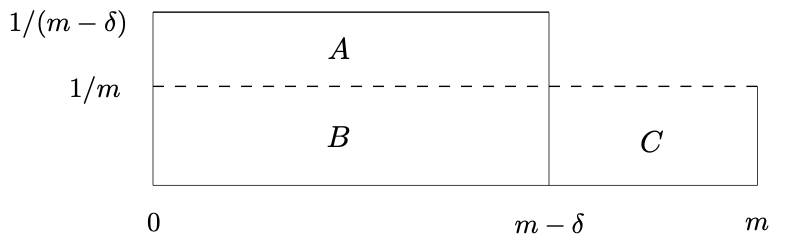
\includegraphics[width=0.55\linewidth]{figures/chapter3/fig-vac1.png}
\end{figure*}

$P_0$ 和 $P_1$ 的统计距离就是图中区域 $A$ 和区域 $C$ 面积和的一半。此外,由于概率分布的总和为 $1$,我们必然有:
\[
\text{area of } B+ \text{area of } A= 1 = \text{area of } B+ \text{area of } C
\]
因此区域 $A$ 和区域 $C$ 的面积相等。所以:
\[
\Delta[P_0,P_1]=\text{area of } A = \text{area of } C ={\delta}/{m}
\]
\end{example}

下面的定理使我们能够在计算上不可区分性和统计距离这两个概念之间建立起联系。

\begin{theorem}\label{theo:3-10}
令 $P_0$ 和 $P_1$ 是有限集 $\mathcal R$ 上的两个概率分布,那么我们有:
\[
\max_{\mathcal{R}'\subseteq\mathcal{R}}|P_0[\mathcal{R}']-P_1[\mathcal{R}']|=\Delta[P_0,P_1]
\]
其中,最大值在 $\mathcal R$ 的所有子集 $\mathcal R'$ 上都能取得。
\end{theorem}

\begin{proof}
假设我们把 $\mathcal{R}$ 分成两个互不相干的子集:由使得 $P_0(r)<P_1(r)$ 的 $r\in\mathcal R$ 组成的集合 $\mathcal{R}_0$,以及由使得 $P_0(r)\geq P_1(r)$ 的 $r\in\mathcal R$ 组成的集合 $\mathcal{R}_1$。考虑下面的 $P_0$ 和 $P_1$ 分布的示意图,其中 $\mathcal{R}_0$ 的元素被放在 $\mathcal{R}_1$ 的元素的左边:

\begin{figure*}[h!]
  \centering
  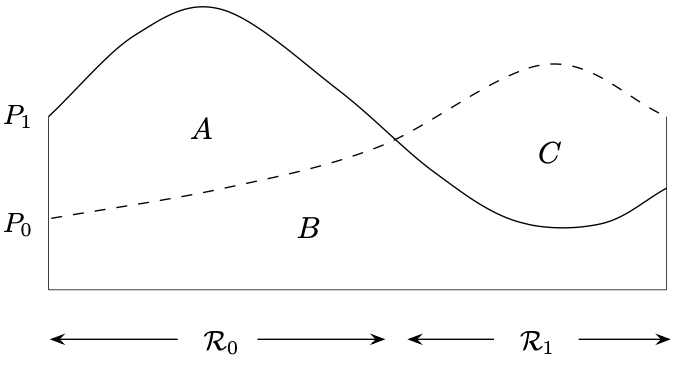
\includegraphics[width=0.45\linewidth]{figures/chapter3/fig-vac2.png}
\end{figure*}

现在,与例 \ref{exmp:3-1} 中一样,我们有:
\[
\Delta[P_0,P_1]=\text{area of } A = \text{area of } C
\]
注意到,对于 $\mathcal{R}$ 的每个子集 $\mathcal{R}'$,我们都有:
\[
P_0[\mathcal{R}']-P_1[\mathcal{R}']=\text{area of } C' - \text{area of } A'
\]
其中 $C'$ 指位于 $\mathcal{R}'$ 上的 $C$ 的子区域,$A'$ 指位于 $\mathcal{R}'$ 上的 $A$ 的子区域。由此可知,当 $\mathcal{R}'=\mathcal{R}_0$ 或 $\mathcal{R}'=\mathcal{R}_1$ 时,$|P_0[\mathcal{R}']-P_1[\mathcal{R}']|$ 取得最大值,此时最大值就等于 $\Delta[P_0,P_1]$。
\end{proof}

与计算上不可分性的联系如下:

\begin{theorem}\label{theo:3-11}
假设 $P_0$ 和 $P_1$ 是有限集 $\mathcal{R}$ 上的概率分布,那么对于任意对手 $\mathcal A$,我们都有:
\[
{\rm Dist\mathsf{adv}}[\mathcal{A},P_0,P_1]\leq\Delta[P_0,P_1]
\]
\end{theorem}

\begin{proof}
考虑一个如攻击游戏 \ref{game:3-3} 中那样试图区分 $P_0$ 和 $P_1$ 的对手 $\mathcal A$。

首先,我们考虑 $\mathcal A$ 是确定性算法的情况。在这种情况下,$\mathcal A$ 的输出是一个 $r\in\mathcal{R}$ 的函数 $f(r)$,它是由挑战者发送给 $\mathcal A$ 的。令 $\mathcal{R}':=\{r\in\mathcal{R}:f(r)=1\}$。如果 $W_0$ 和 $W_1$ 是攻击游戏 \ref{game:3-3} 中定义的两个事件,那么对于 $b=0,1$,我们有:
\[
\Pr[W_b]=P_b[\mathcal{R}']
\]
根据定理 \ref{theo:3-10},我们有:
\[
{\rm Dist\mathsf{adv}}[\mathcal{A},P_0,P_1]=|P_0[\mathcal{R}']-P_1[\mathcal{R}']|\leq\Delta[P_0, P_1]
\]

我们下面考虑 $\mathcal A$ 是概率性算法的情况。我们可以认为 $\mathcal A$ 接受一个辅助输入 $t$ ,代表它的随机选择。我们认为 $t$ 是从某个有限集 $\mathcal{T}$ 中均匀随机选出的。因此,$\mathcal A$ 的输出是挑战者交给它的值 $r\in\mathcal{R}$ 和代表其随机选择的值 $t\in\mathcal{T}$ 的函数 $g(r,t)$。对于一个给定的 $t\in\mathcal{T}$,令 $\mathcal{R}_t':=\{r\in\mathcal{R}:g(r,t)=1\}$。然后,对 $t$ 的随机选择进行平均化,我们有:
\[
\Pr[W_b]=\frac{1}{|\mathcal{T}|}\sum_{t\in\mathcal{T}}P_b[\mathcal{R}_t']
\]
由此可得:
\[
\begin{aligned}
{\rm Dist\mathsf{adv}}[\mathcal{A},P_0,P_1]
&=|P_0[\mathcal{R}']-P_1[\mathcal{R}']|\\
&=\frac{1}{|\mathcal{T}|}\bigg\lvert\sum_{t\in\mathcal{T}}(P_0[\mathcal{R}_t']-P_1[\mathcal{R}_t'])\bigg\rvert\\
&\leq\frac{1}{|\mathcal{T}|}\sum_{t\in\mathcal{T}}|P_0[\mathcal{R}_t']-P_1[\mathcal{R}_t']|\\
&\leq\frac{1}{|\mathcal{T}|}\sum_{t\in\mathcal{T}}\Delta[P_0,P_1]\\
&=\Delta[P_0,P_1]\qedhere
\end{aligned}
\]
\end{proof}

作为该定理的一个结论,我们可以看到,如果 $\Delta[P_0,P_1]$ 可忽略不计,那么 $P_0$ 和 $P_1$ 是计算上不可区分的。

\vspace{5pt}

我们还可以将两个随机变量之间的统计距离定义为它们相应分布之间的统计距离。也就是说,如果 $\mathsf{X}$ 和 $\mathsf{Y}$ 是在一个有限集 $\mathcal{R}$ 中取值的随机变量,那么它们的\textbf{统计距离}是:
\[
\Delta[\mathsf{X},\mathsf{Y}]
:=
\frac{1}{2}
\sum_{r\in\mathcal{R}}
|\Pr[\mathsf{X}=r]-Pr[\mathsf{Y}=r]|
\]
在这种情况下,定理 \ref{theo:3-10} 表明:
\[
\max_{\mathcal{R}'\subseteq\mathcal{R}}
|\Pr[\mathsf{X}\in\mathcal{R}']-\Pr[\mathsf{Y}\in\mathcal{R}']|=\Delta[\mathsf{X},\mathsf{Y}]
\]
其中,最大值在 $\mathcal R$ 的所有子集 $\mathcal R'$ 上都能取得。

类似地,我们还可以对随机变量而非分布来定义区分优势。使用随机变量的好处是,我们可以更方便地处理彼此相关的分布,正如下面的定理所例证的那样。

\begin{theorem}\label{theo:3-12}
如果 $\mathcal{S}$ 和 $\mathcal{T}$ 是有限集,$\mathsf{X}$ 和 $\mathsf{Y}$ 是在 $\mathcal{S}$ 上取值的随机变量,并且 $f:\mathcal{S}\to\mathcal{T}$ 是一个函数,那么 $\Delta[f(\mathsf{X}),f(\mathsf{Y})]\leq\Delta[\mathsf{X},\mathsf{Y}]$。
\end{theorem}

\begin{proof}
对于某个 $\mathcal{T}'\subseteq\mathcal{T}$,我们有:
\[
\begin{aligned}
\Delta[f(\mathsf{X}),f(\mathsf{Y})]
&=|\Pr[f(\mathsf{X})\in\mathcal{T}']-\Pr[f(\mathsf{Y})\in\mathcal{T}']|\quad\text{\emph{(根据定理} \ref{theo:3-10}\emph{\,)}}\\
&=|\Pr[\mathsf{X}\in f^{-1}(\mathcal{T}')]-\Pr[\mathsf{Y}\in f^{-1}(\mathcal{T}')]|\\
&\leq\Delta[\mathsf{X},\mathsf{Y}]\quad\text{\emph{(根据定理} \ref{theo:3-10}\emph{\,)}}\qedhere
\end{aligned}
\]
\end{proof}

\begin{example}\label{exmp:3-2}
令 $\mathsf{X}$ 均匀分布在集合 $\{0,\dots,m-1\}$ 上,$\mathsf{Y}$ 均匀分布在集合 $\{0,\dots,N-1\}$ 上,且 $N\geq m$。令 $f(t):=t\;\mathrm{mod}\;m$。我们想计算 $\mathsf{X}$ 和 $f(\mathsf{Y})$ 之间的统计距离的上界。我们可以这样做。令 $N=qm-r$,其中 $0\leq r<m$,因此 $q=\lceil{N}/{m}\rceil$。同时,令 $\mathsf{Z}$ 均匀分布在集合 $\{0,\dots,qm-1\}$ 上。那么 $f(\mathsf{Z})$ 就均匀分布在集合 $\{0,\dots,m-1\}$ 上,这是因为 $\{0,\dots,m-1\}$ 中的每个元素在函数 $f$ 下都有相同个数的原像(即$q$个),这些原像都落在集合 $\{0,\dots,qm-1\}$ 中。由于统计距离只取决于随机变量的分布,根据定理 \ref{theo:3-12},我们有:
\[
\Delta[\mathsf{X},f(\mathsf{Y})]=\Delta[f(\mathsf{Z}),f(\mathsf{Y})]\leq\Delta[\mathsf{Z},\mathsf{Y}]
\]
正如我们在例 \ref{exmp:3-1} 中所看到的:
\[
\Delta[\mathsf{Z},\mathsf{Y}]=\frac{r}{qm}<\frac{1}{q}\leq\frac{m}{N}
\]
因此有:
\[
\Delta[\mathsf{X},f(\mathsf{Y})]<\frac{m}{N}
\]
\end{example}

\begin{example}
现在我们想要生成一个给定区间 $\{0,\dots,m-1\}$ 上的伪随机数。假设我们有一个PRG $G$,它可以输出 $L$ 比特的序列。当然,一个 $L$ 比特的序列可以被看作是 $\{0,\dots,N-1\}$ 中的一个数,其中 $N:=2^L$。让我们假设 $N\geq m$。

为了生成一个区间 $\{0,\dots,m-1\}$ 上的伪随机数,我们可以把 $G$ 的输出看作是 $\{0,\dots,N-1\}$ 中的一个数,并将其模 $m$ 后输出。我们下面将表明,只要 $G$ 是安全的,且 ${m}/{N}$ 可忽略不计,上述方法所产生的数和从区间 $\{0,\dots,m-1\}$ 中随机挑选的真随机数在计算上不可区分。

为此,令 $P_0$ 为 $G$ 输出并模 $m$ 后的分布,$P_1$ 为 $\{0,\dots,m-1\}$ 上的均匀分布,令 $\mathcal A$ 是一个试图区分 $P_0$ 和 $P_1$ 的对手,就像在攻击游戏 \ref{game:3-3} 中的那样。

令游戏 $0$ 为攻击游戏 \ref{game:3-3} 中的实验 $0$,在这个实验中,$\mathcal A$ 被赋予了一个按照 $P_0$ 分布的随机样本,记 $W_0$ 是 $\mathcal A$ 在游戏 $0$ 中输出 $1$ 的事件。

现在,定义游戏 $1$ 与游戏 $0$ 基本相同,只是我们用一个从区间 $\{0,\dots,N-1\}$ 中随机选出的真随机数代替 $G$ 的输出。记 $W_1$ 为 $\mathcal A$ 在游戏 $1$ 中输出 $1$ 的事件。我们很容易构建出一个有效对手 $\mathcal{B}$,它可以像攻击游戏 \ref{game:3-1} 中那样攻击 $G$,并使得:
\[
{\rm PRG\mathsf{adv}}[\mathcal{B},G]=|{\rm Pr}[W_0]-{\rm Pr}[W_1]|
\]
思路是 $\mathcal{B}$ 获取到它的挑战值并模 $m$,然后将这个值交给 $\mathcal A$,然后原样输出 $\mathcal A$ 输出的任何东西。

最后,我们定义游戏 $2$ 为攻击游戏 \ref{game:3-3} 中的实验 $1$,在这个实验中,$\mathcal A$ 被赋予了一个按照 $P_1$ 分布的随机样本,也就是 $\{0,\dots,m-1\}$ 上的均匀分布。记 $W_2$ 为 $\mathcal A$ 在游戏 $2$ 中输出 $1$ 的事件。如果 $P$ 是游戏 $1$ 中交给 $\mathcal A$ 的值的分布,那么根据定理 \ref	{theo:3-11},我们就有 $|\Pr[W_1]-\Pr[W_2]|\leq\Delta[P,P_1]$;此外,根据例 \ref{exmp:3-2},我们还有 $\Delta[P,P_1]\leq{m}/{N}$。

将以上结论综合起来,可以得到:
\[
\begin{aligned}
{\rm Dist\mathsf{adv}}[\mathcal{A},P_0,P_1]
&=|\Pr[W_0]-\Pr[W_2]|\leq|\Pr[W_0]-\Pr[W_1]|+|\Pr[W_1]-\Pr[W_2]|\\
&\leq{\rm PRG\mathsf{adv}}[\mathcal{B},G]+\frac{m}{N}
\end{aligned}
\]
而根据假设,该值可忽略不计。
\end{example}

\subsection{数学细节}

和之前一样,我们下面会详述相关的数学细节,以便从渐进复杂性理论的角度解释本节的定义和结论。

在定义计算上不可区分性(定义 \ref{def:3-4})时,我们应该考虑两个概率分布族 $P_0=\{P_{0,\lambda}\}_{\lambda}$ 和 $P_1=\{P_{1,\lambda}\}_{\lambda}$,它们都由安全参数 $\lambda$ 索引。对于每个 $\lambda$,分布 $P_{0,\lambda}$ 和 $P_{1,\lambda}$ 都应该在有限比特序列集合 $\mathcal{R}_\lambda$ 中取值,其中 $\mathcal{R}_\lambda$ 中的序列长度以 $\lambda$ 的多项式为界。 在攻击游戏 \ref{game:3-3} 中,安全参数 $\lambda$ 是挑战者和对手的输入,而在实验 $b$ 中,挑战者产生一个根据 $P_{b,\lambda}$ 分布的样本。优势应当被正确地表记为 ${\rm Dist\mathsf{adv}}[\mathcal{A},P_0,P_1](\lambda)$,它是 $\lambda$ 的一个函数,而计算上不可区分性意味着该函数可以忽略不计。

在某些情况下,引入一个概率生成的系统参数可能是很自然的;然而,从技术角度来看,这不是必要的,因为这样的系统参数可以被纳入到分布 $P_{0,\lambda}$ 和 $P_{1,\lambda}$ 中。我们还可以要求 $P_{0,\lambda}$ 和 $P_{1,\lambda}$ 是可有效采样的;然而,为了保持定义的简单性,我们不会强制要求这样做。

统计距离的定义(定义 \ref{def:3-5})从非渐进的角度来看是完全合理的,不需要任何修改或阐述。如前所述,定理 \ref{theo:3-10} 对特定的分布 $P_0$ 和 $P_1$ 成立。定理 \ref{theo:3-11} 可以渐进地看作是说,对于所有分布族 $P_0=\{P_{0,\lambda}\}_{\lambda}$ 和 $P_1=\{P_{1,\lambda}\}_{\lambda}$,对于任意对手(甚至是计算上无界的对手),以及对于所有 $\lambda$,我们都有:
\[
{\rm Dist\mathsf{adv}}[\mathcal{A},P_0,P_1](\lambda)\leq\Delta[P_{0,\lambda},P_{1,\lambda}]
\]